\documentclass[a4paper,UKenglish,compactauthor]{lipics-v2021}
% Remove `screen` option for print version without link colouring


\usepackage[round]{natbib}
\usepackage{microtype}
\usepackage{amsmath}
\usepackage{cleveref}
\usepackage{graphicx}

% Document metadata
\newcommand{\authorName}{Winkler Aron}
\newcommand{\thesisTitle}{Approaches to the automatic detection of
machine-generated text}
\newcommand{\thesisDate}{October 2024}


% Fixing lipics layout
\nolinenumbers
\hypersetup{hidelinks}

% The recommended style is plainurl, but that one does not
% properly work with citet.
\bibliographystyle{abbrvnat}

\EventTitle{Event title}
\EventAuthors{tr-authors}
\EventPublisher{tr-publisher}
\EventLongTitle{tr-title}
\EventShortTitle{MA Thesis}
\EventYear{tr-year}

\title{\thesisTitle}
\titlerunning{\thesisTitle}

\pagestyle{headings}


\begin{document}
%%%%%%%%%%%%%%%%%%%%%%%%%%%%%%%%%%%%%%%%%%%%%%%%%%%%%%%%%%%%%%%%%%%%%%%%%%%%
%%% Title page
%%%%%%%%%%%%%%%%%%%%%%%%%%%%%%%%%%%%%%%%%%%%%%%%%%%%%%%%%%%%%%%%%%%%%%%%%%%%

\begin{titlepage}
  \begin{center}
    {\LARGE Eberhard Karls Universität Tübingen}\\
    {\large Seminar für Sprachwissenschaft \\[4cm]}
    {\huge Master Thesis\\[2cm]}
    {\Large\bf  \thesisTitle\\[1.5cm]}
    {\large \authorName}\\[0.5cm]
    \thesisDate\\[4cm]
    {\small\bf Reviewers}\\[0.5cm]
    \parbox{7cm}%
    {\begin{center}{\large Prof. Dr. Çağrı Çöltekin}\\
        {\footnotesize Seminar für Sprachwissenschaft \\
        Universität Tübingen\vspace{0.4cm}}\end{center}}\hfill\parbox{7cm}%
    {\begin{center}
        {\large Prof. Dr. Gerhard Jäger}\\
        {\footnotesize Seminar für Sprachwissenschaft \\
        Universität Tübingen}\end{center}
    }
  \end{center}
\end{titlepage}

%%%%%%%%%%%%%%%%%%%%%%%%%%%%%%%%%%%%%%%%%%%%%%%%%%%%%%%%%%%%%%%%%%%%%%%%%%%%
%%% Title page reverso
%%%%%%%%%%%%%%%%%%%%%%%%%%%%%%%%%%%%%%%%%%%%%%%%%%%%%%%%%%%%%%%%%%%%%%%%%%%%

\thispagestyle{empty}
\vspace*{\fill}
\begin{minipage}{11.2cm}
  \textbf{\authorName:}\\
  \emph{\thesisTitle}\\ Master Thesis\\
  Eberhard Karls Universität Tübingen\\
  Thesis period: July - November 2024
\end{minipage}
\newpage

%%%%%%%%%%%%%%%%%%%%%%%%%%%%%%%%%%%%%%%%%%%%%%%%%%%%%%%%%%%%%%%%%%%%%%%%%%%%

\pagenumbering{roman}
\setcounter{page}{1}

%%%%%%%%%%%%%%%%%%%%%%%%%%%%%%%%%%%%%%%%%%%%%%%%%%%%%%%%%%%%%%%%%%%%%%%%%%%%
%%% Abstract / Zusammenfassung
%%%%%%%%%%%%%%%%%%%%%%%%%%%%%%%%%%%%%%%%%%%%%%%%%%%%%%%%%%%%%%%%%%%%%%%%%%%%

% The abstract is a short summary of the work to be presented in the thesis
\begin{abstract}
    Recent developments in Natural Language Processing (NLP) have resulted in the development and popularization of highly effective Large Language Models (LLMs), capable of generating convincing and creative linguistic material. LLMs have garnered much attention, both from researchers and the general public, and continue to be increasingly applied to a variety of fields. However, the breakneck speed at which these systems are adopted leaves unattended some of the security concerns regarding their use. Since the language produced by the models is of such high quality, it isn't always feasible to distinguish authentically human contributions from machine-generated text, which can enable a multitude of nefarious applications of LLMs. This work explores the history and inner workings of LLMs, how they can be misused, and possible antidotes to the problem of machine-generated text detection, with a careful eye toward a good balance of computational cost and performance of detection strategies.
\end{abstract}
\newpage



\section*{Acknowledgements}


\cleardoublepage

%%%%%%%%%%%%%%%%%%%%%%%%%%%%%%%%%%%%%%%%%%%%%%%%%%%%%%%%%%%%%%%%%%%%%%%%%%%%%
%%% Table of Contents
%%%%%%%%%%%%%%%%%%%%%%%%%%%%%%%%%%%%%%%%%%%%%%%%%%%%%%%%%%%%%%%%%%%%%%%%%%%%%

% \renewcommand{\baselinestretch}{1.3}

\small\normalsize
\addtocontents{toc}{\protect\setcounter{tocdepth}{0}} % Moronic hack to remove "contents" entry from TOC
\tableofcontents
\addtocontents{toc}{\protect\setcounter{tocdepth}{2}}


% \renewcommand{\baselinestretch}{1}
\small\normalsize

\cleardoublepage


%%%%%%%%%%%%%%%%%%%%%%%%%%%%%%%%%%%%%%%%%%%%%%%%%%%%%%%%%%%%%%%%%%%%%%%%%%%%%
%%% Der Haupttext, ab hier mit arabischer Numerierung
%%% Mit \input{dateiname} werden die Datei `dateiname' eingebunden
%%%%%%%%%%%%%%%%%%%%%%%%%%%%%%%%%%%%%%%%%%%%%%%%%%%%%%%%%%%%%%%%%%%%%%%%%%%%%

\pagenumbering{arabic}
\setcounter{page}{1}

%%%%%%%%%%%%%%%%%%%%%%%%%%%%%%%%%%%%%%%%%%%%%%%%%%%%%%%%%%%%%%%%%%%%
% Content
%%%%%%%%%%%%%%%%%%%%%%%%%%%%%%%%%%%%%%%%%%%%%%%%%%%%%%%%%%%%%%%%%%%%

\section{Introduction}
\label{sec:introduction}

Recent advances in the field of language generation have unlocked the door to the widespread use of language models, across almost all fields of human life -- academics, marketing, arts, programming, and so forth.
For anyone engaging with digital media, talk of generative artificial intelligence (AI) has become a daily occurrence, and many companies are integrating language technology in some form or another.
As it stands, chatbots like ChatGPT and image generators like DALL-E are used by millions to make art, tell exciting stories, improve customer relationships, create tailor-made learning environments for students, and much more.
In this panorama of exciting new technologies, however, there is no lack of worrying signs, and potential for the misuse of these innovative tools.

Language generation has been around since last century, so its massive popularization in 2020 wasn't necessarily as groundbreaking for the discipline as it was for the general public.
What represented the biggest leap was the quality of the output that the language models were capable of.
The generation of material largely indistinguishable from human-written text was available for everyone to use through popular interfaces like ChatGPT.
Given the scale at which AI-generated content has been flooding into all manners of digital phenomena, it has become increasingly crucial to develop up-to-date technologies to detect when a piece of media (for the purposes of this work, only text is considered) is authentically human, or machine-generated.

Language generation has a huge number of positive applications, and it stands to improve people's lives in many ways. Still, the potentially nefarious uses are equally as many.
In fact, even without bad intent, it is easy for model operators to generate and use harmful language in some form.

One example of language models empowering malicious actors is phishing and scamming.
These attacks involve attempting to make their victims reveal sensitive information, or perform certain actions (for example, send money to the attacker or reveal their login information to some service).
Phishing thus far has been (fortunately) plagued by scaling issues -- to increase the number of attacks, one had to hire new human attackers, which is expensive and time-consuming.
With language generation, it could become possible to bypass this limitation by assigning some (or even most) of the work to automated systems.
As models grow more sophisticated, they might become even better suited to gain people's trust for an attacker to exploit, or trick them out of sensitive information outright.

The information landscape, already shaky in the digital age of social media, could also suffer from the malicious employment of language generation.
Disinformation campaigns in the political, social, and commercial spheres have been commonplace throughout human history, but, similar to phishing, have been notoriously expensive to scale.
The ability to generate highly convincing content to further disinforming claims is a great boon to those who seek to spread fabrications and widen divisions.
Worryingly, AI is already being shown to suit the intent to \emph{dis}inform particularly well, to the point that it may even work better as a tool for deception rather than truth.

One need not even intend to harm when employing NLG systems to inadvertently cause damage.
Plagiarism, as an example, is a very real danger with language models, since at any point they may generate one-to-one reproductions of their training data.
On the same note, if the model's training data contained biases and misinformation -- either naturally or as a result of adversarial manipulation -- the generated text could further these without obvious signs or explicit intent.
Chapter \ref{sec:threats} contains further elaboration on these issues, which were only superficially mentioned in this introduction.

In the past, automatic generation of text material relied on relatively simple technologies, and was thus comparatively easier to detect.
The ability to accurately flag generated text could be relied upon with pre-LLM systems, and the quality was often insufficient for the more sophisticated tasks.
Being alerted to the use of AI lessens its danger in most cases -- an inflammatory article is far less effective, a scam email far less convincing, and fake homework much less troublesome when the AI authorship can be reliably exposed.
Unfortunately, starting with GPT-3, not only has the quality of model output grown considerably, but even human evaluators have a tough time separating LM generations from authentic human productions.
Needless to say, automatic detection systems have also suffered a decrease in effectiveness and have had to upgrade their arsenal to keep up.

This thesis aims to delve into the field of machine-generated text detection, exploring the current state of the art, as well as limitations and future possibilities.
Outside of analyzing the various approaches to the problem, this work is meant as a contribution to the development of systems that do not forgo all size concerns in favor of performance.
Modern detection systems rely on models whose running cost is comparable to the massive language models doing the generation -- but the performance gains of this strategy do not necessarily justify the tradeoffs.

When deploying computationally heavy solutions, it is often assumed that they will not run on the end user's machine -- it is after all unreasonable to expect the average user to have hundreds of Gigabytes of RAM on hand.
Instead, the client software is only a relay to the centrally hosted service, with which it communicates over the network.
This may be acceptable in some cases, but it is not desirable in others -- for example, users may and should be reluctant to dispatch their private communications to some remote service in the name of detecting generation.

Fortunately, as with many things, system design is a game of tradeoffs with performance on the one end and complexity on the other.
Highly complex systems, relying on huge models to make predictions, will likely be the best detectors of machine-generated text.
This fact has been true in the field as well as in other areas of computational linguistics: state of the art models often take several GPUs to train and run, with high associated cost.
Still, it is often the case that 80\% of performance can be salvaged at only 20\% of the cost.
This work is written with the somewhat substantiated belief that a version of this proves true in designing solutions for machine-generated text detection as well.

There are many strategies that can be employed to detect machine generation at a reasonable computational costs.
Some examples include pretrained embeddings, which are a valid substitute of contextual embeddings provided by LLMs, and linguistically motivated features, an classical representation of text information that can be computed cheaply.
Task-specific models and even language models are still useful tools.
Not all models are huge, and there is fruitful research of transformer-based models like DistilBERT, which maintain performance close to the original with far fewer parameters.
These methods are discussed in higher detail in Chapter \ref{sec:approaches}.

Target selection is of course important, but customer-facing system designers should aim for standalone solutions that would be able to run on mid-to-high-end machines, when this is feasible.
In this work, a series of options to achieve this are presented, with some of them directly experimented with in the context of Task 8 at SemEval 2023.
The proposed models to detect LM generation employ, among other strategies, GPT-2-based perplexity metrics, linguistically motivated features, pretrained embeddings, contextual embeddings with small models, and task-specific character-level models.
A full discussion of the methods is presented in Chapter \ref{sec:task}.

Note to professor: I plan to write 2-3 more paragraphs here to conclude the introduction more elegantly, but I haven't been able to come up with a version I like yet.
\newpage
\section{Background}

In 1951, Gnome Press published Isaac Asimov's \emph{Foundation} \citep{asimov1951foundation}, the first title of a trilogy that would go on to become one of the cornerstones of modern science fiction.
In the novel, set in the distant future, scientist Hari Seldon predicts the fall of the Galactic Empire, an event that would pave the way to an era of barbarism in the story's fantastical universe.

To preserve humanity's knowledge and technical skills, Hari Seldon establishes the Foundation on an uninhabited planet on the periphery of the Empire, a sort of outpost dedicated to being the home to the archival effort.
The novel follows the political and technological adventures of the Foundation and its leaders, with one of the first plot points being the first conflict between the Foundation and a major local power in the periphery, Anacreon, which declared its independence as the Empire's influence in the periphery weakened.
Seeking protection from the Empire against Anacreon's expansionary stance, the Foundation hosts a diplomatic emissary from the Empire, a Lord Dorwin, finally obtaining a convoluted treaty between the Empire and Anacreon over their respective spheres of influence.

\begin{quote}
    "Before you now you see a copy of the treaty between the Empire and Anacreon – a treaty, incidentally, which is signed on the Emperor's behalf by the same Lord Dorwin who was here last week – and with it a symbolic analysis."

    The treaty ran through five pages of fine print and the analysis was scrawled out in just under half a page.

    "As you see, gentlemen, something like ninety percent of the treaty boiled right out of the analysis as being meaningless, and what we end up with can be described in the following interesting manner:

    "Obligations of Anacreon to the Empire: None!"

    "Powers of the Empire over Anacreon: None!"

    \vspace{0.2cm}

    \begin{flushright}
        \small \emph{Isaac Asimov, Foundation,\\Part II: The Encyclopedists}
    \end{flushright}
\end{quote}

At this point the Foundation's scientists, through a technique they call \emph{"symbolic analysis"}, condense several pages of treaty into a few lines, revealing the hidden meaning behind the layers of legal dissimulation.
By doing so, they expose the inability of the dying empire to exert its influence over its own periphery, and they realize that moving forward, they can only rely on themselves, marking perhaps the true starting point of the story in Asimov's \emph{Foundation}.

Despite first reading this passage when I was a teenager, perhaps over a decade ago, these fictional twists stayed with me through the years.
They were, after all, my first indirect exposure to the field of computational linguistics and natural language processing (NLP).
I remember being mesmerized by the potential of machine computation applied to natural language, in what I would later learn to better define as a mixture of information retrieval and automatic text summarization.

While Asimov's pen definitely hit the mark in predicting some of the most intriguing and successful applications of NLP in the years ahead, what granted computational linguistics perhaps its brightest moment in the limelight was one of its other, albeit related, subfields: language modelling and generation.

\subsection{Language modelling}

Teaching a machine to understand and produce natural language is intuitively a difficult task.
Even if one could reliably collect all ingredients that make up human language, creating a system that emulates it even just well-enough is a very tall order, since there would likely be millions if not billions of cases to consider.
Linguists have documented hundreds of languages, each with their own grammar, peculiarities, exceptions, all of which have yet to be described under one common ruleset.
Manually building a program from the ground up for even just one language is beyond what current technology is capable of.

The very first chatbot, ELIZA \citep{weizenbaum1966eliza}, simulated conversation through pattern matching and substitution, essentially repeating and paraphrasing their interlocutor's statements.
While it successfully bypasses the necessity of programming a machine with \emph{intelligence}, such an approach does not result in a system that can be described as creative in any sense.
In other words, ELIZA will never write a poem, or surprise their conversation partner with a witty turn of phrase.
It would never be able to tell whether May has 30 or 31 days because it has no notion of what \emph{May} and \emph{days} are.
Teaching language is, after all, not only an issue of grammar, but one of world knowledge as well.

If \emph{teaching} language to machines as one would to humans is not possible, and rule-based approaches such as ELIZA inevitably reach a bottleneck, then it becomes necessary to adopt a new strategy, rooted in statistics.
This new approach consists in the realization that the sentence "he's wearing a circumference jacket" is much less likely to be uttered than "he's wearing a yellow jacket".
Extrapolating the pattern, the set of words that can fill the gap in "he's wearing a \_\_\_\_\_ jacket" is varied, but "yellow" will have a much higher \emph{probability} of showing up than "circumference".
Language models are the tools that are employed to estimate these probabilities.

Due to recent innovations in NLP, the phrase "language model" evokes big and expensive systems, trained on huge amounts of data and costing enormous amounts of money to develop.
While this is certainly understandable, the label in itself has no presupposition of size or cost.
In essence, language models, and NLG (Natural Language Generation) systems in general, break down the massively complex problem of "teaching language to machines", into the more manageable task of "statistically learning what words are likely to follow others".
In other words, language models produce next-word (or, more generally, next-token) probabilities based on an input sequence \citep{gao2004introduction}.
After this is achieved, the resulting model can be prompted over and over, one word at a time, in order to generate long pieces of text, by a process called autoregressive generation \citep{lin2021limitationsautoregressivemodelsalternatives}.

For example, for the completion "fifteen minutes of \_\_\_\_\_", one would expect a (good) language model to offer words such as "fame" or "overtime".
One idea to achieve this is to collect some linguistic data and observe what words follow "fifteen minutes of" and extrapolate a probability distribution from the observed frequencies.
So-called \emph{n-gram} language models \citep{chen1999empirical} are built in this fashion, with the \emph{n} in \emph{n-gram} specifying the amount of left context taken into consideration.

The simplest of these models, the bigram (2-gram) language model, records co-occurring word pairs in the sample dataset.
Consequently, for this model, only the last word of a sequence determines the prediction over the following word.
This results in a model that can reliably generate short collocations, such as "Marie \emph{Curie}", but cannot generate coherent sentences, and would likely even fail to offer "fame" as a completion to "fifteen minutes of \_\_\_\_\_", since the only available context for the prediction is the word "of".
To correctly predict "fame", one would need at least a 4-gram language model, which would finally allow for such a "long" context requirement.
However, while taking more context tokens into consideration increases the performance of n-gram language models, it does so at a steep (especially memory) cost: for 4-gram LMs with a vocabulary size (i.e., how many words the model knows) of 1000, for example, implementations without optimizations would require the frequency counts for $10^{4}$ n-grams to be accessible for predictions.

Another issue that presents itself with frequency-based models is the handling of unseen n-grams. For example, the 3-gram "duck goose pony" may never come up in the model training data, in which case some near-0 probability is assigned to the sequence (due to smoothing, see for example \citet{chen1999empirical}).
While some n-grams will fail to appear due to being ungrammatical or nonsensical like in "duck goose pony", others may be perfectly well-formed but either rare or just absent from the training data due to chance: if "trees need hydration" was never observed, then the model would fail to recognize this n-gram to be more likely than, for example, "trees need circumference" (assuming the latter was also not observed, which is quite likely in organic text).
Even the n-gram "roundly faucet knowledge" would be equally as likely as "trees need hydration" if both were never observed in training. While the latter example can be solved by including lower-order n-grams in the probability calculation ("trees need" may have been observed even if "trees need hydration" wasn't, but "roundly faucet" is unlikely to have been observed; see \citet{katz1987estimation}), the former case requires more subtle knowledge.
In order to correctly assess "trees need hydration" as a quite likely n-gram, the model would need to identify the similarity between the words "water" and "hydration", and infer that "trees need hydration" should have higher probability than, say, "trees need virtual", due to "water" and "hydration" being similar.

Due to such limitations, n-gram language models are not the piece of technology that propelled language modelling to the heights that we associate with it today.
The missing piece of the puzzle are neural networks \citep{anderson1995introduction}, which when applied to language generation give rise to \emph{neural language models}.

Following the example above, both n-gram and neural language models solve the fundamental problem of estimating the probability that the word "fate" follows "fifteen minutes of".
However, in order to do so, n-gram language models draw upon explicit frequency observations when generating its output, an approach that often fails to consider an adequate amount of context, or to take into account the fact that similar words appear in similar contexts.
In contrast, neural language models draw upon their internal parameters - the weights and biases \citep{anderson1995introduction} associated to the various layers of the neural network that makes up the model.

\subsection{Neural language modelling}

Neural networks are an extremely powerful for many applications across several disciplines. Providing an effective summary of all neural networks is a difficult task, since they manifest themselves in different variations for different tasks.
Still, they are generally understood as interconnected layers of \emph{neurons} that map an input vector of numbers to an output vector. Each neuron in the network is made up of a vector of weights, a bias, and an activation function, which are used to transform an input vector to an output number.
For the purposes of this work, it is more important to understand the overall network rather than its individual parts: neural models are a way to apply complex transformations to vectors.
The \emph{parameters} of the model, i.e. the combined weights and biases of the individual neurons, can be used to encode knowledge in a way that simpler statistical models struggle to achieve.

Above, the example of "trees need water" and "trees need hydration" was briefly discussed. While n-gram models have no structural way to note the similarity between "water" and "hydration", and thus fail to recognize that the admissible contexts for the two words have some overlap, neural networks have been employed to solve this problem exactly because of their capacity to progressively store knowledge.
Word embeddings \citep{selva2021review} are a way of representing words as numerical vectors, such words with similar semantics will be close to each other in terms of vector distance.  The embeddings for "water" and "hydration" would therefore be closer in vector space than "water" and "dog".
Several ways have been developed to derive embeddings from text data --- for example, the CBOW \citep{mikolov2013efficientestimationwordrepresentations} algorithm uses neural networks to predict the missing word given the surrounding context through the use of a neural network.
For many iterations, the model is presented with a piece of text with a gap, and the objective of guessing the missing item. With each example, the model parameters are updated, or \emph{nudged} in the correct direction (for information on gradient descent, see \citet{zhang2019gradientdescentbasedoptimization}), i.e. towards a state that are more conducive to the correct prediction.
Importantly, among the parameters of the neural network are the embeddings for every word, which are used by the model to compute the final prediction across subsequent layers --- these are random at the beginning, but progressively more and more refined.
At the end of training, most model parameters are discarded, but the embeddings are kept, and hopefully the result will have captured semantic similarities between the entries.

While the CBOW algorithm discards all model parameters aside from the embeddings, it is naturally possible to train the neural model with the objective of keeping all of them, still taking advantage of the architecture's capacity to learn and store information. This is the basis for modern, highly sophisticated language models, with billions or even trillions of parameters.

\subsection{Large Language Models}

Language models have a long and intricate history, having been iterated upon from different perspectives and with different architectural approaches.
The introduction of the transformer \citep{vaswani2023attentionneed}, a model type that for more efficient training over extremely large text data, propelled language model quality forward considerably, to the point that all language models commonly known today follow this architecture.
The ability to train models with relatively little expenses allowed models to grow further and further in perplexity, eventually resulting in what we identify today as Large Language Models (LLMs).
In terms of research attention, BERT \citep{devlin2019bertpretrainingdeepbidirectional} and GPT-2 \citep{radford2019language} have perhaps been the most resonant examples earlier on.

Bidirectional Encoder Representations from Transformers (BERT) is slightly different from the language models discussed so far, in that its primary purpose is not generation.
The word embeddings described above are a powerful tool for obtaining meaningful representations, but have the significant flaw of not being context-aware.
For example, it's clear that the word "honey" should have different embeddings between "bees make honey" and "honey, wake up!".

BERT is a solution to this problem: instead of training a model to then only keep the embedding layer (in other words, computing all embeddings \emph{offline}), BERT is a full-fledged language model that evaluates pieces of text as a whole to return their representations \emph{online}.
As such, when evaluating "bees make honey" and "honey, wake up!" with BERT, "honey" will have vastly different embeddings to account for the different context.

BERT was developed, in other words, to compute context-aware word representations, hence the name. It cannot be used for language generation, mostly because it's nature as a \emph{bidirectional} model.
For the example language model architectures described above, there was an underlying assumption that only the \emph{left} context is visible to the model. This makes intuitive sense: when generating language, only what came before influences the probability distribution of the next word.
This is not the case for BERT. Since the objective here is to evaluate finished productions, BERT may use all previous and subsequent tokens at each timestep.

Despite being a fairly recent introduction to the scene, being made available in just 2018, BERT has made big waves in nearly all fields where processing natural language is even tangentially relevant.
It even resulted in the birth of the somewhat jokingly named discipline of BERTology, which is meant to convey the detailed analysis of how BERT and its different variations exactly arrive at the high-quality embeddings that they are known for.

In the same year as BERT was published, another historical language model also made its debut: OpenAI's GPT-2.
GPT-2 \citep{radford2019language} lines up closer to the popular idea of what constitutes a language model. It is large in size with 1.5 billion parameters, and was primarily conceived for language generation.
In the original paper, the authors highlighted the ability of the model to approach several different problems without explicit training, such as question answering, test summarization, machine translation, and so forth.
In this sense, GPT-2 is one of the first successful examples of language models displaying generalized problem-solving skills, that require both articulation and minute world knowledge.

GPT-2 has become more of a baseline than a challenger in the years following its introduction, such was its impact in research applications. It has garnered much attention and analysis, similarly to BERT, a process that also highlighted some of its flaws (see, for example, the GPT-2 unicorn story\footnote{\url{https://pbs.twimg.com/media/DzYpsJOU0AA1PO9.png:large}}). While talk about GPT-2 could not at all be considered undertone, it was perhaps cut short, in that nowadays it is more rarely employed compared to BERT. This is in large part due to its new iteration, GPT-3 \citep{brown2020language}.

\subsection{Fears and reactions to LLMs}

In 2020, GPT-3 was announced by the company OpenAI, and was made available to the general public through an interface called ChatGPT. With its introduction, the gates were open to the generation of high-quality text through AI.
This was perhaps the first example of language model garnering tremendous general attention, not only in academic circles but from the public at large. ChatGPT even experienced service outages due to its servers not being able to handle the astounding traffic they were receiving.
The introduction of GPT-3 provided an unprecedented boost to language models as a consumer technology, leading to a sort of arms race both in integrating AI into customer-facing products, as well as in model development itself.
In the first wave of AI competition, Facebook's Llama \citep{touvron2023llama} and the open source model Mistral \citep{jiang2023mistral} also entered the scene, alongside Google's now discontinued Bard (see for example \citet{fowler2023bard}). In a subsequent wave, further developments have reached even higher generation quality, with models such as GPT-4 \citep{openai2024gpt4technicalreport} and Gemini \citep{geminiteam2024geminifamilyhighlycapable}.

Such developments marked the beginning of language models being commonplace technology.
The arts, education, technology, sales, and dozens of other fields have seen major changes to the way they operate, either in alongside or in opposition to artificial intelligence.
Education, in particular, was one of the first areas to experience a problematic application of language generation, with a prevailing initial fear that students would opt to have a language model solve their homework for them.
Surprisingly, programming also saw the rapid birth of assistive technology, such as Github Copilot \citep{chen2021evaluatinglargelanguagemodels}, leading to fears that many software professionals would be made obsolete by the new technologies.

People employed in artistic fields, particularly writers, also took a deeply cautious stance from the beginning with respect to AI.
In a landmark development, the 5-month-long strike of the Writer's Guild of America\footnote{An article summarising the strike can be viewed at https://www.vox.com/culture/2023/9/24/23888673/wga-strike-end-sag-aftra-contract}
resulted in an agreement which included safeguards for writers against the use of artificial intelligence\footnote{See for example https://www.nbclosangeles.com/news/local/hollywood-writers-safeguards-against-ai-wga-agreement/3233064/ for an account of the agreement}.
Such a stance turned out to be far from unfounded, with how AI-generated content has flooded several Internet platforms.
As recently as March 2024, even the Google search engine has had to address the issue of unoriginal content, which is in large part meant to target results which contain generated text\footnote{Google published a blog post explaining the changes at https://blog.google/products/search/google-search-update-march-2024/}.
At the same time, the search engine itself adopted a new feature called AI Overviews, an integrated AI-generated response to the user's query\footnote{Google published a blog post explaining its new AI integration at https://blog.google/products/search/generative-ai-google-search-may-2024/}.

The use of large language models thus has been observed to spark mixed reactions, both emotionally and legislatively. However, what was considered so far in this examination is the \emph{lawful} and (perhaps arguably) moral use of language technology.
This does not mean that such technologies cannot be employed with harmful intent --- quite the contrary. the discussion about malicious use of language generation has been left on the sidelines in the early years of LM adoption, but worries are progressively making their way to the forefront of the debate, and countermeasures are becoming increasingly pursued research objectives.
\newpage
\section{Threats posed by NLG systems}
\label{sec:threats}

NLG systems, and language models in particular, have emerged as an extraordinarily useful tool in a number of creative and technical fields, but it stands to reason that they would lend themselves to nefarious applications just as well as ethical ones.
Following \citet{crothers2023machinegeneratedtextcomprehensive}, several threat models \citep{shostack2014security} have been proposed to tackle the potential dangers of language generation, some of which have already had real-life realizations as well.

Threat modelling provides researchers and professionals with the tools to predict potential dangers related to resources or technologies, even (and especially) in absence of historical expertise related to the relevant threats.
For example, when designing a messaging application, a possible exploitation attempt could involve a malicious actor eavesdropping on other users' conversations.
A threat model designed around this scenario would try to define the characteristics of the attacker, the likely strategies used, and how to counter them, preemptively or reactively.
The methodical evaluation of potential threats and the implementation of relevant protection mechanisms is of particular concern in the field of information technology, since this area is so synonymous with scalability.
Indeed, when something goes wrong in systems that operate on a huge scale, as do many if not most digital services people interact with daily, the impact is often proportionally disastrous.

NLG systems integrate themselves into this picture better than one might initially assume.
Importantly, language models scale far more easily than a human force. Humans need to be taught, few at a time and for a period of time, to perform a task.
Automated systems, however, have no such limitation: once trained, one must only increase the compute to increase coverage, an operation that takes far less time and resources than training people.

As such, language generation makes the known universe of digital threats that much more severe.
On the one hand, it boosts the scale at which already existing attacks were operating, such as scams and phishing attempts - both of which had to be performed by human actors in some way thus far.
On the other hand, it creates entirely new threats which were previously unfeasible, such as generating convincing documents for homework-evasion.

\subsection{Scam and phishing attempts}

Attacks and exploitation attempts targeted at individuals are particularly well-suited for NLG usage, since they usually involve using natural language to convince the victim of performing some action, such as revealing sensitive information or granting access to a restricted resource.

Phishing is a cyberattack method where attackers impersonate legitimate entities to trick individuals into revealing private information, such as passwords, credit card numbers, or personal details.
This is typically done through deceptive emails, messages, or websites that appear trustworthy but are actually fraudulent. Victims are often lured into clicking malicious links or downloading harmful attachments, leading to the theft of their data or the compromise of their devices.
Phishing is a widespread and dangerous tactic used to gain unauthorized access to systems and conduct identity theft, financial fraud, or other malicious activities.

An example of a phishing attack could involve a fake email that appears to come from a well-known bank. The email might use the bank's logo, official-sounding language, and a convincing sender address to create a sense of urgency, such as warning the recipient that their account has been compromised.
The message instructs the recipient to click on a link to verify their account information immediately. When the user clicks the link, they are directed to a counterfeit website that looks almost identical to the bank's real site.
Once on this fake site, the victim is prompted to enter their login credentials, which are then captured by the attackers.
With this information, the cybercriminals can access the victim's real bank account, potentially leading to financial loss and identity theft.

NLG has been proven to be effective across several varieties of phishing attacks. Depending on the scope of the attack, one can distinguish phishing attacks targeting indiscriminate groups (massive phishing), specific communities (community phishing) or individuals in particular (spear phishing).

Regarding the former, the exploitation attempt targets a specific group or community, such as members of a social club, employees of a particular company, or even residents of a neighborhood. The attacker leverages the shared characteristics, interests, or affiliations of the community to create a more convincing and believable scam.
For instance, a cybercriminal might send an email that appears to come from the community’s leader, such as a club president or company CEO, announcing an upcoming event or an urgent matter requiring action.
The message may ask recipients to click on a link to RSVP, pay dues, or access important information.
This link, however, leads to a fraudulent website designed to capture login credentials, financial details, or other sensitive information.
By exploiting the trust and familiarity within the community, these phishing attacks can be particularly effective, as victims are more likely to lower their guard and engage with the malicious content.

E-mail masquerade attacks are among the most common and most well-studied \cite{Khonji2013PhishingDA} digital vectors for phishing attacks.
Language generation has been studied in correlation to them even before GPT-3 came to the forefront, and has been shown to be effective at creating a variety of attacking strategies with only few hours of effort \cite{bakie2017scaling}.
Aside from providing an important method to scale up email-based attacks, language generation also renders traditional spam and phishing filters less effective.

One of the most widely used method for distinguishing legitimate emails from spam is Bayesian filtering. This approach works by analyzing each word in an email and comparing it against a database of words commonly found in spam messages.
The filter calculates the probability of the email being spam based on the presence and frequency of these words. If the likelihood exceeds a certain threshold, the email is flagged as spam.
Despite some shortcomings, such as being vulnerable to adversarial manipulation of the underlying frequency tables, Bayesian filtering remains an effective tool for detecting and blocking unwanted emails.

NLG systems could throw a wrench in this common approach, since large language models are capable of higher and less predictable lexical variety than traditional NLG systems.
Community Targeted Phishing, as described by \citet{Giaretta_2019} aims explicitly to analyze the language of specific groups to craft complex emails, which with the help of today's LLMs can more easily evade traditional defenses.
For example, a conversational LM could be trained on the style and publications of a well-known researcher, to then be used as a phishing actor against colleagues in the same area, who may not be directly familiar with the renowned figure.
This clone may much more convincingly get victims to surrender personal information and click on malicious links, while evading.

The more dangerous variety of phishing attacks, however, is \emph{spear phishing}. Spear phishing focuses on a single individual, using personalized information gathered from research to craft a highly convincing and tailored attack.
This makes spear phishing more difficult to detect, as the attacker often impersonates someone the target knows or trusts, increasing the likelihood of success.
The personalized nature of spear phishing often leads to greater harm, as the attacker aims to extract highly sensitive information or gain unauthorized access to critical systems.

The bigger limitation of these attacks -- from the perpetrator's perspective -- is that much time investment and human time is needed for each target.
NLG systems could provide a tool for scaling such attacks, for example by being employed in early stages for automated conversations, thus gaining the victim's trust before the attack proper.

The language generation features provided by modern LLMs thus pose a substantial threat when it comes to their ability to boost the effectiveness of phishing attacks.
Their ability is well suited to tricking large groups of people indiscriminately, as well as to strategies that prove insidious to threaten specific communities.
They also enable the scaling up of phishing attacks targeted at individuals, since they can engage in conversation, preparing the field for the malicious extraction of sensitive information.
The industry's tools for protection against traditional attacks are rendered somewhat obsolete when LLMs enter the picture, thus effectively detecting when a language model is being deployed is crucial.

\subsection{Information poisoning}

Generating Sentiment-Preserving Fake Online Reviews Using Neural Language Models

AI and the Future of Disinformation Campaigns

\subsection{Faking human authorship}

Prevalence of nonsensical algorithmically generated papers in the scientific literature

Is GPT-3 Text Indistinguishable from Human Text? Scarecrow: A Framework for Scrutinizing Machine Text
\newpage
\section{Previous approaches}
\label{sec:approaches}

If the above foray into the threat models concerning language generation that have been discussed in research has revealed anything, it is that expecting model operators to disclose the nature of texts submitted to their recipients is a naive and potentially dangerous habit.
Thankfully, as language models have grown larger and more sophisticated, so have strategies and technologies detecting them matured alongside them.
Though it has certainly received and influx of manpower interest since then, automatic detection of machine generated text has been an active area of research even from before 2020 -- after all, as was previously discussed, there was no shortage of attempts to exploit NLG technologies well before the recent GPT craze.

In Chapter \ref{sec:background}, this thesis presented an overview of different ways in which text could be represented, on a spectrum ranging from surface-level metrics to neural contextual embeddings.
Many parallels can be drawn between these strategies and the methodologies employed to detect machine generation.
In the following sections, several well researched and tested detection strategies will be explored, some taking advantage of linguistically motivated features or even frequency-based metrics, while others lean into the times and use LLMs themselves to discriminate between authentic and generated productions.
It should however be underlined that the movement toward more sophisticated vectorization processes does not necessarily entail a one-sided improvement across all possible aspects involved in the detection pipeline.

On the contrary, moving up the ladder of complexity comes at the cost of requiring increasing amounts of computational power.
Such approaches are extremely valid explorations of what is the best that can be achieved, but applicability in the real world is often limited since the end users cannot run the required software on commonplace commercial machines.
Separating the application into client and server, which is the common approach taken in other AI fields, is only acceptable in the narrower subset of cases which have no privacy requirement regarding the data being verified.
Chapter \ref{sec:task} will dive deeper into the more "cheap" approaches, meaning those that forgo heavy systems, aiming instead to strike a balance between performance and (compute) accessibility.

\subsection{Frequency and feature-based methods}

\begin{enumerate}
    \item https://arxiv.org/abs/1904.09751
    \item https://peerj.com/articles/cs-443/
    \item https://ieeexplore.ieee.org/abstract/document/9892269
    \item https://ieeexplore.ieee.org/abstract/document/8282270
    \item https://arxiv.org/abs/2111.02878
\end{enumerate}

\subsection{Neural approaches}

\begin{enumerate}
    \item Adversarial Robustness of Neural-Statistical Features in Detection of Generative Transformers
    \item Defending against neural fake news
    \item Cross-Domain Detection of GPT-2-Generated Technical Text
    \item Real or Fake? Learning to Discriminate Machine from Human Generated Text
    \item DetectGPT: Zero-Shot Machine-Generated Text Detection using Probability Curvature
\end{enumerate}


\subsection{Domain differentiation}

\begin{enumerate}
    \item Technical: Cross-Domain Detection of GPT-2-Generated Technical Text
    \item Socials:  Automatic Detection of Bot-Generated Tweets
    \item Socials, reviews: Detecting computer-generated disinformation
    \item Socials: Deep Fake Recognition in Tweets Using Text Augmentation, Word Embeddings and Deep Learning
    \item Chatbots:  Detecting Bot-Generated Text by Characterizing Linguistic Accommodation in Human-Bot Interactions
    \item Ecom: Creating and detecting fake reviews of online products.
\end{enumerate}
\newpage
\section{Task 8 at SemEval 2024}
\label{sec:task}

The 18th International Workshop on Semantic Evaluation (SemEval-2024) was a large event in NLP, offering various challenges that teams across the world could undertake.
Task 8 at SemEval-2024 \citep{wang2024semeval} centered around machine-generated text detection in a black-box setting (i.e., the generator models for the test set were not known while the competition was ongoing), in both monolingual and multilingual components.

This shared task spanned 3 subtasks: subtask A a binary classification task between generated and human texts, subtask B consisted in multi-class classification between multiple LLM generators, as well human texts, while subtask C was a boundary detection problem, where participants had to correctly pinpoint the boundary between a human and a machine-generated segment in each test.
During the active phase of SemEval-2024, which ended in February 2024, I undertook Task 8 jointly with Daniel Stuhlinger, a fellow student at the University of Tübingen.
The full report of our participation, carried out under the team name "TueCICL", can be viewed in \citet{stuhlinger-winkler-2024-tuecicl}.

As team TueCICL, we submitted results for two of the subtasks to the leaderboards, namely subtask A and subtask C, which were the two subtasks involving classification between solely human and machine-generated texts, whereas subtask B focused more on inter-generator differentiation.
For subtask A, consisting in binary classification over the whole texts, there were two phases development, one for shared task proper, and subsequent post-deadline experimenting in the context of this Master Thesis.
Due to the more pronounced research interest in subtask A, as well as to better present the higher volume of material associated with it, this section shall first discuss subtask C, then dive deeper into subtask A later in this Chapter.

\subsection{Human - LM Boundary detection}

Subtask C of the shared task addresses detection environments that are characterized by active adversarial agents performing the generation.
Specifically, detection technologies have been observed to be weak to techniques also found in obfuscation \citep{macko2024authorship}, such as paraphrasing \citep{krishna2024paraphrasing} and noise-introduction \citep{wang2021adversarial}.
Change point detection, which is the titular requirement of subtask C, addresses another way in which the use of NLG technology might be obfuscated.
In the scenario targeted by the subtask, a human segment ranging from 0\% to 50\% of the text is concluded by a machine-generated component, making the text as a whole much harder to flag as a generation.

Task organizers provided generations by GPT variants and the LLaMA series \citep{touvron2023llama}, but unfortunately not in high abundance: the training set around 5000 texts, and was accompanied by development set containing a little over 500 more.
Table \ref{fig:taskc_data} offers an overview of the data distribution across the sets.
Alongside the general scarcity of training and cross-validation data, one should also note that a relevant portion of the data is entirely machine-generated, meaning the change index is exactly 0.
Though this of course preserves the objective of being able to reliably detect fully generated texts, it does cut into the already low amount of true change examples available in training.

The evaluation metric by which the submitted solutions are measured is Mean Absolute Error (MAE), i.e. the average absolute difference in the predicted change-point index and the true value.
The baseline suggested by the organizers was based on Longformer \citep{beltagy2020longformerlongdocumenttransformer}, a RoBERTa checkpoint specialized in long texts.
This baseline achieved an impressive 3.5 MAE on the development set -- a tough standard -- and a (much lower) 21.54 MAE on the test set, though the latter was of course not known at development time.

\vspace{1cm}

\begin{table}[h]
    \centering
    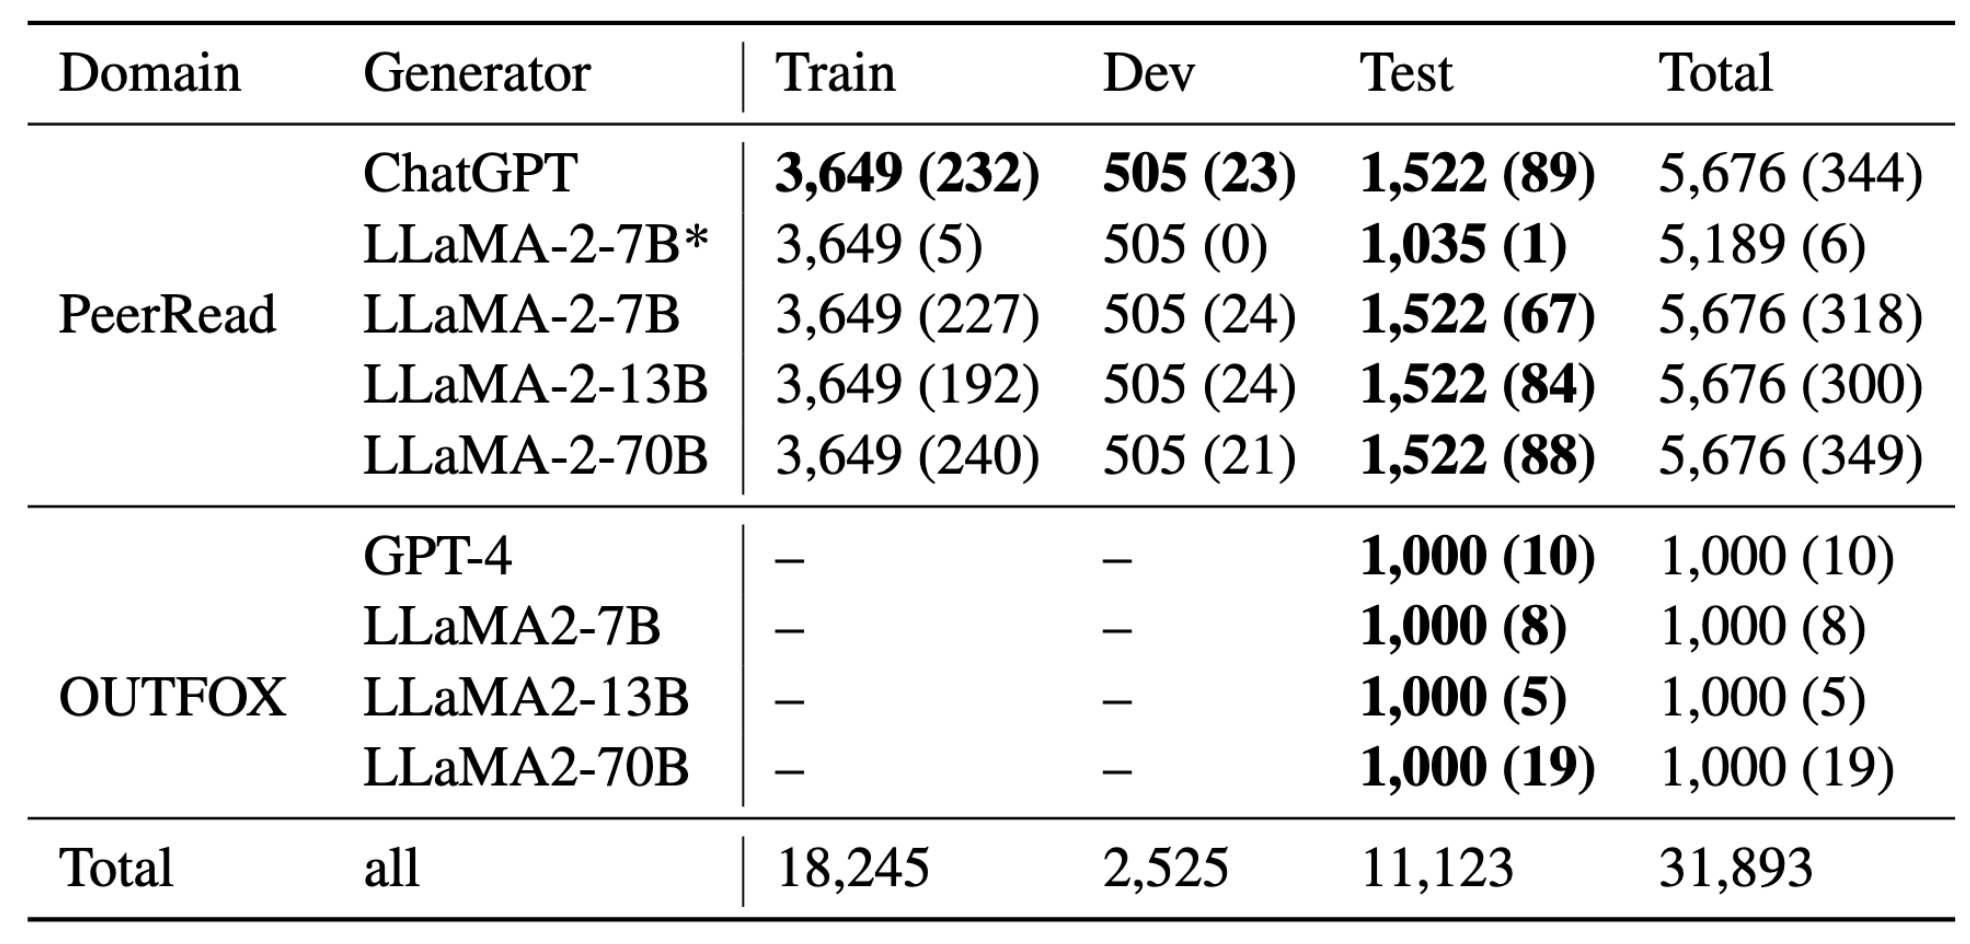
\includegraphics[width=0.7\textwidth]{assets/subtaskc-data.png}
    \caption{
        Dataset breakdown for subtask C from Task 8 at SemEval-2024.
        The number in “()” is the number of examples purely generated by LLMs, i.e., human and machine boundary index=0.
        LLaMA-2-7B* and LLaMA-2-7B used different prompts. Bold data is used in shared task training development, and test.
    }
    \label{fig:taskc_data}
\end{table}

Following the example set by the baseline, the solutions we devised did not attempt to predict the boundary change index directly -- instead, we performed binary classification at the token level, essentially asking whether any given token belongs to the human or the machine-generated segment.
In accordance with the general mission of producing solutions that could run on at least midrange home computers and laptops, large-scale transformer-based approaches, such as the one provided as the baseline, were discarded altogether.

Instead, we presented an ensemble model sourcing its input from two bidirectional long short-term memory, or LSTM \citep{hochreiter1997long}, models.
The first LSTM operated at the character level and did not include any elements of pertaining.
Preprocessing the input texts for this character-level model involved lowercasing, and mapping numerals and punctuation to a \verb|<NUM>| and a \verb|<PUNCT>| special token respectively.
Similarly, whitespace characters of any type (e.g. space, tab, newline) were also mapped to the special token \verb|<WS>|.
Classification then proceeds as outlined on the character level, and the first occurrence of the positive label (indicating that the token belongs to the machine segment) is taken as the boundary change index.
Naturally, the character-level index is traced back to the word-level position, as required by the task setting, where the position of the word in which the first positively classified character is located is taken as the final label.

The second LSTM relied on pretrained Word2Vec \citep{mikolov2013efficientestimationwordrepresentations} embeddings sourced from the Wiki2Vec project \citep{yamada2020wikipedia2vec}. Static embeddings have fallen out of favor lately due to the emergence of contextual embeddings derived from LLMs, but they offer the significant advantage of not requiring firing up a large language model at inference time, a property that made them well-suited for our objectives in subtask C.
While this LSTM performs word-level classification, as opposed to the character-level nature of the first model, many of the preprocessing steps are maintained.
Casting texts to lowercase letters is all the more relevant since the Word2Vec mapping is case sensitive, and also maintained mapping numerals, punctuation and white-space to special tokens.

At least on paper, employing pretrained Word2Vec embeddings introduces an important amount of information into the model that would not be possible to obtain solely based on the available training data.
However, for the character-level LSTM, there are no such mitigating factors.
From very early on, it was clear from intermediate results that the character-level LSTM struggled significantly, since it had no pretrained semantic context for the input letter sequences.
To address this excessive burden placed on the scarce training data to both inform on how human language works, as well as how to distinguish it from generations, we enrich the dataset provided for subtask C with that of subtask A.
While deep discussion of the latter is reserved for the later sections of this chapter, it should suffice to say that training data for subtask A contains over 100.000 records, providing ample, linguistic material, albeit not targeted to the specific objective of subtask C.

Records imported from the training set for subtask A had the target label set to either 0 (for fully machine-generated texts), or the length of the tokenized text (for fully human texts).
Since this operation carries the inevitable side effect of drowning out the far fewer examples where a change occurs mid-text (which are available in subtask C's data only), all models are trained for 5 epochs on the enriched data, and then on the original task data.
Aside from the aforementioned optimizations, hyperparameter tuning over the characteristics of the models yielded that, for both LSTM's, a hidden size of 512 and 2 layers resulted in the highest validation performance.

After training the two base approaches, an ensemble model was also constructed combining the representations of the two LSTM's.
This consisted in a non-recurrent feed-forward network (FFN) whose inputs were the concatenated representations at the word level.
For the character-level model, this meant averaging the representation at every character for any given word.
Utilizing a simple FFN in this case was deemed to be the most efficient solution, since the interaction between the various elements of the sequence is already captured in the sub-model.
This is also similar to how token-level classification is performed with transformers, with a feed-forward classification head applied at each token.
The best-performing hidden size for this model was found to be 256.
Table \ref{tab:c_models} offers a summary of the models developed for subtask C.

\begin{table}[h]
    \centering
    \begin{tabular}{llll}
        \hline
        \textbf{Model}  & \textbf{Type} & \textbf{L*} & \textbf{H**} \\
        \hline
        Character-level & LSTM          & 2           & 512          \\
        Word2vec        & LSTM          & 2           & 512          \\
        Joint model     & FFN           & -           & 256          \\
        \hline
        \vspace{0.1cm}
    \end{tabular}
    \caption{Summary of models for subtask C. \textbf{*} Number of layers. \textbf{**} Hidden size.}
    \label{tab:c_models}
\end{table}


\subsection{Generated text detection}
\label{subsec:subtask_a}

\subsection{Generated text detection: post-deadline additions}
\newpage
\section{Discussion of SemEval results}
\label{sec:discussion}

\subsection{Subtask A: Shared Task analysis rankings}

\begin{table}[ht]
    \centering
    \begin{tabular}{llll}
        \toprule
        \textbf{Model}     & \textbf{Development set} & \textbf{Test set} & \textbf{Ranking} \\
        \midrule
        Baseline           & 0.72                     & 0.88              & 20               \\
        \midrule
        Character-level    & 0.85                     & 0.55              & 127              \\
        Word2vec*          & 0.82                     & 0.72              & 85               \\
        Language features* & 0.63                     & 0.88              & 21               \\
        Joint model*       & 0.83                     & 0.69              & 96               \\
        \bottomrule
        \vspace{0.1cm}
    \end{tabular}
    \caption{Results for SemEval-2024 Task 8, subtask A. Dev and Test columns report the accuracy on the respective data partitions. The ranking column refers to the model ranking in the shared task competition. The scores and ranking of the unofficial submissions were not provided by the organizers and computed by team TueCICL. There was a total of 137 submissions.\\ \textbf{*} unofficial submissions}
    \label{tab:a_results}
\end{table}

Table \ref{tab:a_results} shows the results for each model submitted during the proceedings of the shared task, for subtask A.
On the development set, almost all models outperform the transformer baseline provided by the organizers.
The best performing model was the character-level model, with an accuracy of 0.85 -- this was our final submission for the shared task.
While the two recurrent models and the joint model do not differ very much from one another, the FFN built on linguistically motivated global feature vectors sets itself apart in that it is the worst performing model on the development set.

Perhaps the most important lesson here is that there's clearly diminishing returns in closely fitting the development set -- perhaps even negative returns, as the worst-performing model in development is the best-performing one on the test set by a big margin.
At any rate, it wouldn't be honest to put the blame of this middling performance on the development set alone.
Selecting character-level and Word2Vec-based solutions appears after the fact to have been a misfire as well.
For further information, the original task report \citep{stuhlinger-winkler-2024-tuecicl} contains an in-depth rundown of the shared task, while the following pages are dedicated to how these lessons can help improve performance on the task, with little adjustments to the methods, that nonetheless preserve the mission of computationally efficient, locally runnable detectors.

\subsection{Subtask A: post-deadline improvements}

Having taken note of the disappointing performance of the official submissions to the shared task, a new batch of experiments was conducted in the context of this Master Thesis.
These had the objective of being more firmly grounded in research, while still maintaining the objective of developing detectors which end-users would be able to own and run on their own machines.
A new approach was developed, targeting generator models one at a time with different strategies, since machine-generated detection seems to be an elusive target when targeting all generators at once.
Instead, the work was split among many different classifiers, attempting to differentiate between human texts and only one generator (Davinci, ChatGPT, Cohere, Dolly, BLOOMz).

The first batch of experiments resulted in the single-generator classifiers described in Table \ref{tab:subsolutions-initial}.
Among these models was the one showing the best ever performance on the test set, with an 89\% classification accuracy by the TF-IDF model on Davinci, though this model would have been impossible to find without access to the test set labels, since its performance on the development does not stand out.
After running the full experiment, which ended in the development of the ensemble model, it was also observed that the approach resulted in good, but not excellent classification performance.
Table \ref{tab:ensemble-initial} describes the two ensemble models, one neural and one trained with a random forest base.
Unfortunately, neither ensemble beats the baseline, and both fall short of the best single-generator classifier on the test set.
They also both underperform the best unofficial submission to the shared task, which was developed by team TueCICL, achieving 88\% test set accuracy with only linguistically motivated features.

Chapter \ref{sec:task} concluded with the description of the last experimental run, which followed the general lines of the first, with a re-sampled development set.
The single-generator model lineup was also extended to include the three BLOOMz classifiers, one with a fine-tuned DistilBERT model, and two statistical approaches with TF-IDF and language feature representations respectively.
The remainder of this section is dedicated to the analysis of this last experimental run, which resulted in a final ensemble with a classification accuracy of 97\% on the test set.

The first task in the newly formulated approach to the task of machine-generated text detection is obtaining a set of single-generator classifiers.
As a reminder, a total of 15 such classifiers, one for each model and strategy combination, are trained on a subset of the train data, containing only human texts and generations from the target model.
The validation set for these models is constructed along the same lines, containing no generations from other models, to ensure each single-generator classifier is selected based solely on its ability to detect its target.
Probability scores associated to the positive label are then used as input to the final ensemble classifier.


\begin{table}[ht]
    \centering
    \vspace{0.1cm}
    \begin{tabular}{llp{10px}ccp{10px}c}
        \toprule
        \multirow{2}{*}{Model} & \multirow{2}{*}{Strategy} &  & \multicolumn{2}{c}{Development set} &               & Test set                   \\
                               &                           &  & \tiny{Preicision}                   & \tiny{Recall} &          & \tiny{Accuracy} \\
        \midrule
        ChatGPT                & DistilBERT                &  & 1.00                                & 0.66          &          & 0.83            \\
        ChatGPT                & TF-IDF                    &  & 0.97                                & 0.55          &          & 0.88            \\
        ChatGPT                & Language Feats            &  & 0.98                                & 0.69          &          & 0.83            \\
        Davinci                & DistilBERT                &  & 0.95                                & 0.82          &          & 0.77            \\
        Davinci                & TF-IDF                    &  & 0.94                                & 0.68          &          & 0.89            \\
        Davinci                & Language Feats            &  & 0.97                                & 0.87          &          & 0.97            \\
        Cohere                 & DistilBERT                &  & 0.96                                & 0.82          &          & 0.69            \\
        Cohere                 & TF-IDF                    &  & 0.94                                & 0.66          &          & 0.70            \\
        Cohere                 & Language Feats            &  & 0.96                                & 0.65          &          & 0.45            \\
        Dolly                  & DistilBERT                &  & 0.87                                & 0.92          &          & 0.62            \\
        Dolly                  & TF-IDF                    &  & 0.89                                & 0.81          &          & 0.87            \\
        Dolly                  & Language Feats            &  & 0.99                                & 0.30          &          & 0.56            \\
        BLOOMz                 & DistilBERT                &  & 0.92                                & 0.10          &          & 0.55            \\
        BLOOMz                 & TF-IDF                    &  & 0.80                                & 0.32          &          & 0.54            \\
        BLOOMz                 & Language Feats            &  & 0.70                                & 0.57          &          & 0.56            \\
        \bottomrule
        \vspace{0.1cm}
    \end{tabular}
    \caption{
        Performance metrics for final single-generator classifiers.
        The development set referenced here is the one derived from the train set and described in Chapter \ref{sec:task}, not the original development set.
        Precision and recall refer to the \textbf{positive} label, not to the average of the metric over the two classes.
    }
    \label{tab:subsolutions-final}
\end{table}

The objective for single-generator classifiers is to be as specialized as possible in detecting generations from a single model.
In other words, they should be geared towards high precision, rather than high recall.
Table \ref{tab:subsolutions-final} provides a summary of the single-generator classifiers, with precision and recall for the positive label (i.e. for the machine-generated class) over the re-sampled development set, and accuracy on the test set.
There are several takeaways from this table that are worth mentioning.
Initially, it can be noted that precision is high for nearly all classifiers, which is in concordance with the models' training goals.
For some single-generator classifiers, even the recall value for the positive label is respectable, meaning that the models display good ability to detect generations from other models as well.
Another interesting aspect is that for all generators, at least one strategy displays high precision, even when other strategies struggle.
For example, BLOOMz-targeted models struggle when using TF-IDF and language features, but are rescued by their DistilBERT sibling.
Similarly, detectors for Dolly in the TF-IDF and DistilBERT strategies do not inspire high confidence, but the features-based classifier appears to have specialized much more than the others, and could come to the rescue for difficult scenarios despite its low test-set performance.
Feature-based detectors generally perform above expectations, with all except BLOOMz developing a highly specialized toolkit, resulting in especially high precision.
In this sense, they are perhaps the strategy that best captures the objective of the single-generator models: highly specialized systems, that can detect one specific model with very high precision.
As will be seen later, this is likely why they are a crucial driver for performance in the ensemble classifiers.

When it comes to performance on the test set, the results of course do not differ from those already reported in Table \ref{tab:subsolutions-initial}, since these are the same models, evaluated on the same data.
For the 12 single-generator classifiers that were already discussed, only the precision and recall metrics were new introductions to the conversation.
In that sense, the metrics paint a positive picture, with a good degree of specialization among models, with high precision being an indicator of success even in the face of low test-set accuracy.
The BLOOMz-targeted models were trained with only 1500 positive examples, with a further 1000 reserved for validation.
Predictably, this led to the non-pretrained models being at a disadvantage, since TF-IDF and feature-based models need more data than fine-tuning to achieve a good fit.
Indeed, the DistilBERT-based detector is the best-performing classifier in terms of precision, with the two other models lagging behind.
The scarcity of data appears to have hurt the features-based classifier the most, even though this strategy is very high-performing when detecting other generators.
Not only is the fine-tuned classifier the most precise, but it also appears to be the most highly specialized.
It achieved a recall of only 10\%, which one might mistakenly consider to be a negative measurement.
BLOOMz texts were only responsible for 3\% of generations in the re-sampled development set, meaning that the low recall measured for this model is a positive sign of highly optimized detection behavior, which again is the goal of the single-generator classifiers.
The TF-IDF and feature-based classifiers for BLOOMz do not display similar behavior, as their lower precision and higher recall indicate that they take more shots in the dark, which constitutes and undesirable, if perhaps inevitable outcome.
If any conclusion is to be drawn from the results in Table \ref{tab:subsolutions-final}, it would be that the process has seemingly produced at least one highly specialized detector for all generators, with some less precise but hopefully good auxiliary models.
It remains to be seen whether it is possible to obtain an ensemble that properly leverages the properties of the single-generator models.

Aside from verifying the models' performance on their own targets, it should also help to check in more detail how well these classifiers generalize to unknown generators.
Table \ref{tab:generalization} presents generalization metrics for the same models as above.
Each value in the table represents the recall score, i.e., the proportion of documents from a particular generator that a model correctly flagged as machine-generated, with detector-generator model concordance being bolded.

\begin{table}[ht]
    \vspace{0.1cm}
    \centering
    \begin{tabular}{llccccc}
        \toprule
        Model   & Strategy           & ChatGPT       & Davinci       & Cohere        & Dolly         & BLOOMz        \\
        \midrule
        ChatGPT & DistilBERT         & \textbf{1.00} & 0.74          & 0.68          & 0.39          & 0.15          \\
        ChatGPT & TF-IDF             & \textbf{1.00} & 0.64          & 0.43          & 0.25          & 0.13          \\
        ChatGPT & Language Features  & \textbf{1.00} & 0.60          & 0.50          & 0.86          & 0.03          \\
        Davinci & DistilBERT         & 0.99          & \textbf{0.99} & 0.78          & 0.63          & 0.47          \\
        Davinci & TF-IDF             & 0.85          & \textbf{1.00} & 0.60          & 0.40          & 0.27          \\
        Davinci & Language Features  & 0.94          & \textbf{1.00} & 0.87          & 0.90          & 0.23          \\
        Cohere  & DistilBERT         & 0.96          & 0.80          & \textbf{1.00} & 0.68          & 0.27          \\
        Cohere  & TF-IDF             & 0.66          & 0.59          & \textbf{1.00} & 0.51          & 0.35          \\
        Cohere  & Language Features  & 0.71          & 0.69          & \textbf{1.00} & 0.35          & 0.16          \\
        Dolly   & DistilBERT         & 0.98          & 0.86          & 0.97          & \textbf{0.99} & 0.53          \\
        Dolly   & TF-IDF             & 0.78          & 0.73          & 0.83          & \textbf{1.00} & 0.57          \\
        Dolly   & Language Features  & 0.23          & 0.04          & 0.00          & \textbf{1.00} & 0.13          \\
        BLOOMz  & DistilBERT         & 0.01          & 0.03          & 0.03          & 0.02          & \textbf{0.99} \\
        BLOOMz  & TF-IDF             & 0.18          & 0.25          & 0.36          & 0.24          & \textbf{1.00} \\
        BLOOMz  & Language Features  & 0.00          & 0.16          & 0.08          & 0.10          & \textbf{1.00} \\
        \midrule
        ChatGPT & Statistical Tandem & \textbf{1.00} & 0.77          & 0.75          & 0.88          & 0.16          \\
        Davinci & Statistical Tandem & 0.98          & \textbf{1.00} & 0.94          & 0.92          & 0.39          \\
        Cohere  & Statistical Tandem & 0.86          & 0.79          & \textbf{1.00} & 0.65          & 0.39          \\
        Dolly   & Statistical Tandem & 0.79          & 0.74          & 0.83          & \textbf{1.00} & 0.65          \\
        BLOOMz  & Statistical Tandem & 0.18          & 0.34          & 0.39          & 0.30          & \textbf{1.00} \\
        \bottomrule
        \vspace{0.1cm}
    \end{tabular}
    \caption{
        Generalization metrics for each single-generator classifier.
        The reported value is equal to the ratio of correctly flagged documents for a generator, over all documents produced by that generator.
        In other words, a measure of recall is shown for each detector-generator combination.
        Bolded values refer to instances where the detector is trained on the productions of the generator.
        Statistical tandem indicates a combination of the Features and TF-IDF models, where a correct classification by either is counted as a success.
    }
    \label{tab:generalization}
\end{table}

Unsurprisingly, self-detection performance (bolded values) is the best in every case, showing that models are most effective at detecting text generated by the model they were trained on.
On the contrary, cross-model generalization is inconsistent, but there is much more differentiation between models in this case.
For example, ChatGPT detectors generalize moderately well to other models, especially when using the fine-tuning strategy (e.g., 0.68 on Cohere and 0.74 on Davinci).
On the other end of the spectrum, Dolly and BLOOMz detectors perform significantly worse when detecting texts from other generators.
For example, the BLOOMz detector using DistilBERT has almost negligible recall on ChatGPT (0.01) and Cohere (0.03), while Dolly-trained models using language features have very low recall scores on all other generators (e.g., 0.23 for ChatGPT).
In general, the BLOOMz targeted models barely generalize at all, but this is understandable given the low amount of training data.
But more importantly, other models also generalize very poorly to BLOOMz generations, with the best recall being 0.53 (excluding, for now, the tandem models), achieved by Dolly on TF-IDF.
Considering that the test set is made up by around 9\% of BLOOMz models, and that the first attempt at the ensemble strategy did not have BLOOMz-optimized detectors, it is easy to see how that segment of the test set could have ended up mostly misclassified in the first iteration.
Even though the BLOOMz detectors generalize poorly, they still clearly capture something about the generations by their target model (and, hopefully, the class of generators to which BLOOMz belongs in general) that all other classifiers fail to.

DistilBERT models distinguish themselves as the best-generalizing models across the board, especially those targeting ChatGPT and Davinci.
One possible explanation might be that these OpenAI models are either the largest or the most general-purpose models, thus their properties extend father away, whereas other models like Dolly describe themselves as instruction-tuned, thus making their characteristics potentially less general.
In addition, the Davinci and ChatGPT-based detectors share an interesting asymmetrical relationship, where Davinci detectors generalize very well to ChatGPT generations, but not vice versa.
This might also be explained in the context of the degree to which the model is close to the original concept of a general-purpose language model.
Davinci, in essence GPT-3, can be used for all types of completions, whereas ChatGPT is optimized as a chatbot, and takes specialized input prompts as a result.
Another standout performance is the DistilBERT classifier trained on Dolly generations, which boasts high recall on all other generators except BLOOMz.
The TF-IDF variant of the same detector loses a large chunk of recall across the board, and the feature-based classifier impresses with its ability \emph{not} to generalize.
It is important that some detectors show generalization to unknown generators, as this is after all a black-box detection task, where the test set contains a model not seen during training, namely GPT-4.
At the same time, a detector can also contribute by being excellent at detecting only its target, since it would be pointless to aim for unknown generators at the cost of dwindling prediction power over known ones.
The picture painted by Table \ref{tab:generalization} is of a good balance between the two specializations.

\begin{table}[ht]
    \vspace{0.1cm}
    \centering
    \begin{tabular}{lcc}
        \toprule
        Composition            & Development accuracy & Test accuracy \\

        \midrule
        TF-IDF only            & 99.527\%             & 87.179\%      \\
        Language features only & 98.777\%             & 85.466\%      \\
        DistilBERT only        & 96.250\%             & 74.790\%      \\
        TF-IDF + features      & 99.927\%             & 95.544\%      \\
        Full Model             & 99.892\%             & 97.106\%      \\
        \midrule
        Winning model          & NA                   & 96.88\%       \\
        \bottomrule
        \vspace{0.1cm}
    \end{tabular}
    \caption{
        Summary of final ensemble performance across different configurations.
        The best-performing model is the full ensemble, beating the task-winning model, whose reported accuracy is included for comparison.
    }
    \label{tab:ensemble-final}
\end{table}

\subsection{Subtask C: Shared task analysis and rankings}
\newpage
\section{Conclusion}
\label{sec:conclusion}

This Master Thesis has attempted to tackle the problem of machine-generated text detection through the lens of a marked attention to model efficiency and size.
The early chapters served to introduce the field and language modelling in general, hopefully helping to initiate those who were so far unfamiliar with the topic.
Chapter \ref{sec:threats} provided an overview of thread models relating to NLG technologies, such as their potential harmful uses in misinformation campaigns, phishing, or false research.
This was meant as justification for the development of detection technologies: it would be wishful thinking to assume that all actors -- regardless of background, competence, or intention -- will disclose their use of language generation, but alerting users that they're dealing with machine text remains critical.
Following up on the outlined threats, Chapter \ref{sec:approaches} outlined some of the most recent detection approaches present in the scientific literature.
These range from statistical strategies relying on classical representations such as word-frequency vectors and TF-IDF, to solutions employing the same large language models in the detection effort.
Aside from the lively research landscape surrounding the field, especially in recent years, another development that was important to highlight was the movement towards increasingly heavy detection systems.
LLMs and other large transformer-based approaches are responsible for the latest state-of-the-art performance, but these architectures also trade often minor gains for compute requirements that relegate the usage of these solutions to dedicated servers, precluding end users from locally executing software they rely on.

The principal objective of this Master Thesis is to contribute to the conversation surrounding detection systems by proposing alternative solutions that approximate SOTA performance while maintaining a lean model constitution.
The battlefield of choice was Task 8 at SemEval-2024 \citep{wang2024semeval}, a shared task built around black-box detection of machine generated text.
Model development targeting the shared task took place in roughly two stages: the first while SemEval-2024 was ongoing, resulting in official submissions to the leaderboards under the banner of team TueCICL, and a later phase in the context of this Thesis.

The models submitted to the task spanned to subtasks, one consisting in binary classification (subtask A) and the other in change point detection (subtask C).
For both subtasks, the approach was to build an ensemble combining representations from a character-level mode, a TF-IDF model, and a third model build on linguistically motivated features.
This effort resulted in middle-of-the pack rankings, as the submitted solutions fell short of the baseline in both instances, and did not show the convincing performance they exhibited in development.

The second phase of development carried on the work on subtask A, a competition track that challenged participants in pure binary classification over human and machine-generated texts.
Having drawn valuable lesson from the experience during the shared task, and with a more firm grounding the latest research, a new batch of models was developed.
The major introduction in the new stage was to split up the general problem of machine-generated text detection into several sub-problems, aiming to determine whether a target text had been generated by some particular model.
Fifteen single-generator classifiers were trained, three for each of the five models that were included in the data provided for the shared task.
Of the three single-generator classifiers targeting each LLM, one was obtained by fine-tuning DistilBERT, and the other by fitting a random forest classifier with either TF-IDF vectors or linguistically motivated feature representations.
These models were then combined into an ensemble model, which processed each target text by computing the probability that it had been generated by each of the single-generator classifiers, then applying a feed-forward network on the obtained 15-feature vector representation.
This ensemble displayed performance above the task-winning model, and even an ensemble variant that did not have the transformer-based components achieved accuracy levels that would nearly have placed it on the podium.
These results strongly support the argument brought forward by this Thesis, i.e. that there exist answers other than huge transformers along the development of high-performing systems.

Team Genaios \citep{sarvazyan-etal-2024-genaios} submitted the system they named LLMixtic, the solution that won the shared.
This model combined token-level probabilistic features extracted with LLaMA-2 models, placing it firmly in the LLM-based category.
Compared to this formulation, the model proposed in this Thesis achieves more than comparable performance with only DistilBERT as a transformer-based module, a much smaller model family than Facebook's LLaMA.
Even without DistilBERT, model performance remains high, albeit lower than would be required for the shared task podium.
TF-IDF and especially linguistic features bring another advantage to the table: since the resulting representation is tied to surface-level, conceptually solid aspects, such as the frequency and rarity of a unigrams and bigrams, or some linguistic aspect such as POS-tag distributions, it is possible to trace the final prediction back to these characteristics of the input text.
Even though there weren't any explainability analyses carried out in this work, it is in theory possible to extend the simple binary classification with a natural language reason as to \emph{why} a particular decision was made.

Of course, the comparison with the task-winning model offered by team Genaios is not a very fair one, since test set labels were not available during the shared task.
The model proposed in this work was not developed in the dark, and the possibility to check performance on the test set was used multiple times to determine if an acceptable end result had been reached.
There is a popular saying in the digital space, that hindsight is 20-20, meaning literally that it has perfect eyesight in both eyes.
This phrase describes the follow-up experiments rather aptly: there was a wealth of experience around what had work and what hadn't, and a better solution could be built on top of well-understood failures.
This of course only means that the comparison to team Genaios is not exactly correct -- in fact, their achievement, considering the difficulty of the shared task, is more impressive -- but doesn't take away from the final results that were observed.

There are also other limitations to the approach outlined in this Thesis, which should be mentioned.
One such aspect has to do with the composition of the test set.
Referring back to Table \ref{table:adata}, one can note that there are two aspects that make the test set perhaps not an accurate representation of the potential real-world detection landscape.
First, the only new model introduced by the test set is GTP-4, which has two of its predecessors in the train set (ChatGPT and Davinci-003).
In addition, the test partition contains documents sourced from only one domain: student essays from Outfox \citep{koike2024outfox}.
On the one hand, this puts into question exactly how well do proposed models perform in the black-box context, since it can be argued that the "surprise generator" introduced in the test set may not be very surprising.
On the other, while the Outfox data was not present in either partition other than the test set, it is still only one domain, which makes doesn't necessarily translate to other generation contexts.
Some domains in which detecting generation may be critical, but that are not present in this dataset, are e-mails (for example related to phishing and scamming attempts), product or place reviews, or general digital content generations, such as blogs or articles, which may be used in disinformation campaigns.

Another limitation of this work is the absence of additional tests concerning adversarial robustness.
Machine-generated text detection is a field particularly characterized by the race between detectors and evaders.
As detection mechanisms become more sophisticated, there comes a growing incentive to develop strategies to evade detection, for example to bypass AI checks that are being rolled out in academic software to ensure that students do not cheat.
Other research \citep{Crothers_2022} has found that statistical features, such as the language metrics included in this study, help the model resist adversarial attacks, since language features are less easily perturbed than LLM embeddings.
The ensemble model presented in this work would benefit from checks to its adversarial robustness, at least to verify if there's a benefit in this area from employing statistical features.

On this note, future research on this model should explore performance on other datasets, as well as in downstream application with real-world users, since it was designed with true deployment in mind.
Another avenue of experimentation could come from updating or adding modules to the ensemble.
Aside from TF-IDF, linguistic features, and DistilBERT, other useful information sources might come from other similar-sized, but differently tuned language models.
Instruction-tuned or chat-based models could provide valuable feedback in more interactive applications, and auxiliary systems augmented with information retrieval, capable of comparing the suspected generation against a corpus of available information, might take the degree of factuality of the target text in consideration when outputting a prediction.
A more competently set-up character-level model approach may also be more informative than the official results in subtask A might suggest -- after all, the ensemble components more closely associated with style, TF-IDF and language features, performed very well in the post-deadline experiments.
There may be more value to be extracted from the characters, especially since they are more commonly paired with convolutional networks in research, whereas they were used alongside an LSTM in this work, an architecture that is not as well-equipped to deal with the long sequence lengths that come with character-level representations.
In addition, the shared task itself contains two interesting directions that were not explored in relation to this ensemble model.

Subtask C of the shared task consisted in change point detection, a detection scenario in which a human author provides the first part of the text, which is then completed by an AI agent.
The use of NLG is harder to detect in this setup, thus making this strategy common in adversarial evasion techniques.
Drawing from the lessons in the simpler binary classification task, more work could be dedicated to change point detection.
Some of the linguistic features do not translate well, which is a challenge, since moving from a global to a per-token or per-subsequence measure is not equally easy for all representations.
Nonetheless, there's little doubt that future contributions to the field cannot afford to simplify their worldview to one in which a text is either fully generated, or fully not.

Alongside the monolingual, English-only dataset, subtask A had a multilingual variant as well.
This parallel subtask was barely mentioned in this work, since it wasn't undertaken in the official submissions, and the post-deadline additions failed to address it.
However, LLMs are not used only in English -- in fact, cross-linguistic and cross-task performance is one of the evaluation metrics for modern language models.
Smaller models, such as the one proposed in this work, may struggle as the definition of the problem they're solving grows wider -- but this is the exact problem ensembling smaller solutions was meant to address.
As the winning team for the multilingual track, team USTC-BUPT \citep{guo2024ustc} also use a bipartite strategy: after detecting the language of the text, they use a classification head over LLM embeddings for English, and a fine-tuned mT5 variant with a classification token for all other languages.
There is no reason why the specialists that are combined to form the ensemble in this work couldn't be extended to include classifiers for other languages.
The ways in which such an interplay of modules could be architected are extremely diverse and certainly entice a model designer's creativity.

While more work remains to be done in the field of machine-generated text detection, this Master Thesis has successfully shown that incremental adoption of LLMs and other similarly huge models is not the only frontier left to explore.
Solutions designed to run locally may be regarded as fringe solutions in the current landscape, but may become critically important in the future.
Research in this direction may not produce the highest-performing state-of-the-art systems, but it will certainly cover the many use cases in which detection software cannot be offered as a remote service.
Though different researchers and developers are bound to have different views in what they regard as interesting and innovative, there's also a point to be made in favor of the creativity inherent in making the most of whatever resources are available, as opposed to picking the latest off-the-shelf transformer model and fine-tuning it on the latest data collection.
Putting together a system that may be odd and wonky at the start and taking it off the ground offers a sense of achievement if it succeeds and a wealth of lessons when it fails, only to the benefit of end users.


%%%%%%%%%%%%%%%%%%%%%%%%%%%%%%%%%%%%%%%%%%%%%%%%%%%%%%%%%%%%%%%%%%%%%%%%%%%%%
%%% Bibliography
%%%%%%%%%%%%%%%%%%%%%%%%%%%%%%%%%%%%%%%%%%%%%%%%%%%%%%%%%%%%%%%%%%%%%%%%%%%%%
\cleardoublepage

\bibliography{anthology,custom,semeval} % link bibliography.bib


\cleardoublepage
%%%%%%%%%%%%%%%%%%%%%%%%%%%%%%%%%%%%%%%%%%%%%%%%%%%%%%%%%%%%%%%%%%%%%%%%%%%%%
%%% Selbständigkeitserklärung
%%%%%%%%%%%%%%%%%%%%%%%%%%%%%%%%%%%%%%%%%%%%%%%%%%%%%%%%%%%%%%%%%%%%%%%%%%%%%
\thispagestyle{empty}
\section*{Selbständigkeitserklärung}

Hiermit versichere ich, dass ich die vorliegende Masterarbeit
selbständig und nur mit den angegebenen Hilfsmitteln angefertigt habe und dass alle Stellen, die dem Wortlaut oder dem
Sinne nach anderen Werken entnommen sind, durch Angaben von Quellen als
Entlehnung kenntlich gemacht worden sind.
Diese Masterarbeit wurde in gleicher oder ähnlicher Form in keinem anderen
Studiengang als Prüfungsleistung vorgelegt.

\vskip 3cm

Ort, Datum	\hfill Unterschrift \hfill
%%%%%%%%%%%%%%%%%%%%%%%%%%%%%%%%%%%%%%%%%%%%%%%%%%%%%%%%%%%%%%%%%%%%%%%%%%%%%
%%% Ende
%%%%%%%%%%%%%%%%%%%%%%%%%%%%%%%%%%%%%%%%%%%%%%%%%%%%%%%%%%%%%%%%%%%%%%%%%%%%%

\end{document}
